% !Tex root = checkedc.tex

\chapter{Bounds declarations for variables}
\label{chapter:tracking-bounds}

Variables with \arrayptr\ types that are used to access
memory must have bounds declared for them.  The same requirement
holds for variables with incomplete checked array types.
The bounds will be used to check
memory accesses at runtime involving the pointers stored in the variable
or pointers produced by pointer arithmetic that uses those pointers.
Runtime checks can be omitted if a compiler proves that they are
redundant. In addition, for performance-critical code, checks will be
omitted when programmers demonstrate at compile-time that the checks are
redundant (see Section~\ref{section:avoiding-bounds-checks} for details).

\section{Bounds declarations}
\label{section:bounds-declarations}

Bounds are declared using bounds declarations. Bounds declarations have
the form:

\begin{tabbing}
\var{bounds}\=-\var{decl:} \\
\> \boundsdecl{\var{x}}{\var{bounds-exp}} \\
\\
\var{bounds}\var{-exp:} \\
\> \boundscount{\var{non-modifying-exp}} \\
\> \bounds{\var{non-modifying-exp}}{\var{non-modifying-exp}} \\
\> \boundsunknown \\
\> \boundsany
\end{tabbing}

where \var{x} is a variable. Additional forms for handling
\void\ pointers and casts are described in 
Sections~\ref{section:pointers-to-void} and \ref{section:pointer-cast-results}.

A bounds expression describes the memory that can be accessed using the
value of \var{x}, provided that x is not null. Bounds expressions
include counts, pairs that specify an upper bound and lower bound,
\boundsunknown, and \boundsany:

\begin{itemize}
\item
  \boundsdecl{\var{x}}{\boundscount{e1}} describes the number of
  elements that are accessible beginning at \var{x}. Only memory that
  is at or above x and below \var{x} \code{+} \var{e1} can be
  accessed through \var{x}, where \var{x} \code{+} \var{e1} is
  interpreted using \arrayptr\ pointer arithmetic.
\item
  \boundsdecl{\var{x}}{\bounds{\var{e1}}{\var{e2}}}
  describes the range of memory that can be accessed through \var{x}.
  Only memory that is at or above the location specified by \var{e1}
  and below \var{e2} can be accessed through \var{x}.
\item
  \boundsdecl{\var{x}}{\boundsunknown} declares that \var{x} has bounds that
   are unknown at compile-time.
  It is a compile-time error to attempt to access memory using a
  variable of type \arrayptr\ with unknown bounds.
\item
  \boundsdecl{\var{x}}{\boundsany} is a special form that readers can
  ignore for now. It is used for null pointers (0 cast to a pointer
  type) and means that \var{x} can have any bounds. Because null
  pointers cannot be used to access memory, they can have any bounds.
\end{itemize}

Bounds expression use ``non-modifying'' expressions. These are a subset
of C expressions that do not modify variables or memory. They include
local variables, parameters, constant expressions, casts, and operators
such as addition, subtraction, and address-of. 
Section~\ref{section:non-modifying-expressions}  describes
non-modifying expressions in detail.

In a bounds declaration of the form \boundsdecl{\var{x}}{\var{bounds-exp}},
\var{x} can have an \arrayptr\ or a checked array type.
For the form  \boundsdecl{\var{x}}{\boundscount{\var{e1}}},  the type of
\var{x} cannot be \arrayptrvoid\ and the type of \var{e1} must be an integral type.
The usual C integer conversions are applied to \var{e1}.\footnote{If the
type of \var{e1} is a character, a short integer, a bit field, or an enumeration type,
the expression is promoted to an \keyword{int} type if that is large
enough to  hold all values of the type or an \keyword{unsigned int} type otherwise.}
For \boundsdecl{\var{x}}{\bounds{\var{e1}}{\var{e2}}}, \var{e1} and
\var{e2} must be pointers to the same type.  Typically \var{x} is also 
a pointer to that type or an array of that type.  
However, \var{x} can be a pointer to or an array of a different type.
This is useful for describing the results of casts and
bounds for \arrayptrvoid\ pointers.

For any variable with a bounds declaration, the variable must be
non-null when memory is accessed.  There is no requirement that an
\arrayptr\ variable stay within its bounds. The requirement is
that the \arrayptr\ variable can only be dereferenced if it is
in bounds. This avoids bound checks on pointer arithmetic.

Count expressions have limits on their ranges to prevent signed integer
overflow and unsigned integer wraparound from affecting size
computations. Section~\ref{section:integer-overflow-informal}
explains these limits in detail. The limits
depend on the element type of the \arrayptr\ and the type of the count
expression. For \boundsdecl{\var{x}}{\boundscount{\var{e1}}}, where \var{x}
has type \arrayptrT\,
\var{e1} must be greater than or equal to 0. \var{e1} must be less
than the maximum number of \arrayptrT\ elements
that can be indexed by an integer whose type matches that of \var{e1}.
For \ntarrayptr, there is
an null terminator at or beyond the upper bound, so \var{e1}
must be less than the maximum number of \arrayptrT\ elements minus one.

A bounds declaration \boundsdecl{\var{x}}{\boundscount{\var{e1}}} is an
abbreviation for \boundsdecl{\var{x}}{\bounds{\var{x}}{\var{x} \code{+} \var{e1}}} with additional conditions that \var{e1}
\lstinline|>= 0 &&| \var{e1} \lstinline|<= (char *)|
\var{ub}. \var{ub} is either
\lstinline|UINTPTR_MAX/sizeof(|\var{T}\lstinline|)| or
\lstinline|INTPTR_MAX/sizeof(|\var{T}\lstinline|)|.

The conditions may require programmers to add additional checks at memory allocations
to show that \var{e1} is in range. However, the conditions have advantages too.
They provide scaffolding for proving that expressions based on
element counts of \arrayptr\ variables do not overflow or wraparound.

The meaning and correctness of bounds are based on the C semantics for
pointers and pointer arithmetic. At runtime, any non-null pointer in C
has an object associated with it. The association starts when a pointer
is created by a memory allocation operation, address-of expression, or
conversion of an array variable to a pointer-typed expression. It flows
through to pointers that result from pointer arithmetic. At runtime, the
bounds for a pointer must be the bounds of the object associated with
the pointer or a subrange of those bounds. The correctness of declared
bounds information at compile-time is ensured by making allocation sites
and address-of expressions be creators of bounds information and by
propagating bounds with the pointers with which they are associated.
Bounds can be narrowed during propagation, but they cannot be widened.

The meaning of a bounds expression can be defined more precisely. At
runtime, given an expression \var{e} with a bounds expression
\bounds{\var{lb}}{\var{ub}}, let the runtime
values of \var{e}, \var{lb}, and \var{ub} be \var{ev}, \var{lbv},
and \var{ubv}, respectively. The value \var{ev} will be \code{0} (null) or
have been derived via a sequence of operations from a pointer to some
object \var{obj} with \bounds{\var{low}}{\var{high}}.
The following statement will be true at runtime:
\var{ev} \lstinline@== 0 || (@\var{low} \lstinline|<=| \var{lbv} \lstinline|&&|
\var{ubv} \lstinline|<=| \var{high}\lstinline|)|. In other words, 
if \var{ev} is null, the bounds
may or may not be valid. If \var{ev} is non-null, the bounds must be
valid. This implies that any access to memory where \var{ev}
\lstinline|!= 0 &&| \var{lbv} \lstinline|<=| \var{ev} \lstinline|&&| \var{ev}
\lstinline|<| \var{ubv} will be within the bounds of \var{obj}.

In this chapter, to simplify the description, it is assumed that none of
the \arrayptr\ variables that have bounds declarations have
their addresses taken. It is also assumed that the values of variables
whose addresses are taken are not used in bounds declarations. It is
acceptable to use the address of an address-taken variable in a bounds
declaration. This is provided that the resulting address is not used to
access memory in the bounds declaration (that is, indirectly access the
value of a variable). For example, given the declaration \code{int x},
the expression \code{&x} may appear in a bounds expression.  
Chapter~\ref{chapter:pointers-to-data-with-arrayptrs} extends the
design to avoid these restrictions.  It covers pointers to data with 
\arrayptr\ values,  pointers to variables used in bounds, and bounds 
that use pointers.

\section{Using bounds declarations}

Bounds declarations may be added to declarations and statements using
\keyword{where} clauses. They also may be placed inline at a declaration
by following the declarator with \code{:} \var{bounds-exp}. In that
case, the bounds expression applies to the variable that is the subject
of the declarator. By making the bounds be part of the program, this
preserves the control and efficiency of C. The bounds declarations will
be checked statically for correctness using rules described in 
Chapter~\ref{chapter:checking-bounds}.

\subsection{Bounds declarations at variable declarations}
\label{section:variable-declarations}

Here are some examples of bounds declarations as part of variable
declarations. The first function sums the integers stored in memory
between \code{start} and \code{end}, where the integer stored at
\code{end} is not included.

\begin{lstlisting}
int sum(array_ptr<int> start : bounds(start, end), array_ptr<int> end)
{ 
    int result = 0;
    array_ptr<int> current : bounds(start, end) = start;
    while (current < end) {
       result += *current++; // *current is bounds-checked.  The checking ensures 
                             // that current is within the bounds of (start, end) 
                             // at the memory access.                           
    }
    return result;
}
\end{lstlisting}

This can be written using \keyword{where} clauses as well, at the
inconvenience of typing variable names twice in declarations:

\begin{lstlisting}
int sum(array_ptr<int> start where start : bounds(start, end), 
        array_ptr<int> end)
{ 
    int result = 0;
    array_ptr<int> current where current : bounds(start, end) = start;
    while (current < end) {
       result += *current++;                          
    }
    return result;
}
\end{lstlisting}

This function searches for an integer in an array. If it finds the
integer, it returns the index in the array where the integer occurs.
Otherwise, it returns -1.

\begin{lstlisting}
int find(int key, array_ptr<int> a : count(len), int len)
{
    for (int i = 0; i < len; i++) {
         if (a[i] == key) { // a[i] is bounds checked.  The checking
                            // ensures that i is between 0 and len.
             return i;
         }
    }
    return -1;
}
\end{lstlisting}

If the code was written assuming that it would always find the integer,
bounds-checking would detect the buffer overrun in the case the integer
was not present:

\begin{lstlisting}
int bad_find(int key, array_ptr<int> a : count(len), int len)
{
    int i = 0;
    while (1) {
        if (a[i] == key) { // The bounds check will fail when i == len
            return i;
        }
        i++;
    }
    return -1;
}

\end{lstlisting}

This function adds two arrays of 2x2 arrays.

\begin{lstlisting}
int add(int a checked[][2][2] : count(len), int b checked[][2][2] : count(len), 
        int len) 
{
    for (int i = 0; i < len; i++) {
        // All array accesses are bounds checked
        a[i][0][0] += b[i][0][0]; 
        a[i][0][1] += b[i][0][1];
        a[i][1][0] += b[i][1][0];
        a[i][1][1] += b[i][1][1];
    }
}
\end{lstlisting}

Externally-scoped variables can have bounds as well:

\begin{lstlisting}
// external-scoped variables that hold a buffer and its length
int buflen = 0;
array_ptr<int> buf : count(buflen) = NULL;

int sum(void)
{
    int result = 0;
    for (int i = 0; i < buflen; i++) {
        result += buf[i]; // bounds checked
    }
    return result;
}
\end{lstlisting}

This is a declaration of a function that copies bytes provided that the
pointers and lengths are aligned:
\begin{lstlisting}
int aligned_memcpy(array<char> dst where dst : count(len) && 
                                         aligned(dst, 4),
                   array<char> src where src : count(len) && 
                                         aligned(src, 4),
                   int len where len % 4 == 0);
\end{lstlisting}

The declaration can be shortened using in-line bounds declarations to:

\begin{lstlisting}
int aligned_memcpy(array<char> dst : count(len) where aligned(dst, 4),
                   array<char> src : count(len) where aligned(src, 4),
                   int len where len % 4 == 0);
\end{lstlisting}

This example is adapted from the OpenSSL library. The signature of a
method has been modified to have bounds declaration. The size of input
and output buffers must be multiples of 16 because the function operates
on 16-byte chunks of data.

\begin{lstlisting}
void AES_cbc_encrypt(array_ptr<const unsigned char> in : count(len),
                     array_ptr<unsigned char> out : count(len),
                     size_t len where len % 16 == 0,
                     ptr<const AES_KEY> key,
                     array_ptr<unsigned char> ivec : count(16),
                     const int enc);
\end{lstlisting}

\subsection{Bounds declarations for return values}

Bounds may be declared for the value returned by a function. The
parameter list can be followed by either \code{:} \var{bounds-exp} or
a \keyword{where} clause. The special variable \keyword{return\_value} can
be used to refer to the return value. The parameters are considered in
scope for the bounds declaration or \keyword{where} clause. Any parameters
occurring in the return bounds declaration or \keyword{where} clause may
not be modified by the body of the function.

The following example show the \code{find} function from
Section~\ref{section:variable-declarations} modified
to return a pointer to the element instead of the index:

\begin{lstlisting}
array_ptr<int> find(int key, array_ptr<int> a : count(len), int len)
 : bounds(a, a + len)
{
    for (int i = 0; i < len; i++) {
         if (a[i] == key) { // a[i] is bounds checked.  The checking
                            // ensures that i is between 0 and len.
             return &a[i];
         }
    }
    return NULL;
}
\end{lstlisting}

This also can be written as:

\begin{lstlisting}
array_ptr<int> find(int key, array_ptr<int> a : count(len), int len)
  where return_value : bounds(a, a + len)
{
   ...
}
\end{lstlisting}
Here is the declaration of a function that allocates memory:

\begin{lstlisting}
array_ptr<char> alloc(size_t size) : count(size);
\end{lstlisting}



\subsection{Bounds declarations at statements}
\label{section:statement-declarations}

Programmers may wish to delay initializing variables or may wish to
change the bounds of a variable in the middle of a function. This can be
done using bounds declarations attached to expression statements. In C,
an expression is converted to a statement by placing a semi-colon after
the expression. This creates an expression statement. A \keyword{where}
clause may be added before the terminating semi-colon of an expression
statement.

Any variable that has bounds declared at an expression statement has
dataflow-sensitive bounds throughout the body of the function. Only
automatic variables can have bounds declared for them at expression
statements. It does not make sense to have dataflow-sensitive bounds for
externally-scoped variables and variables with static or thread storage.
The bounds extend to the next assignment to any variable in the bounds
declaration, with some exceptions for pointer incrementing or
decrementing. Section~\ref{section:extent-of-declarations} 
describes the extent of flow-sensitive bounds
in more detail.

Here is a simple example that illustrates bounds declarations at
statements. The variable \code{tmp} first points to an array with 5
elements and then points to an array with 10 elements; the bounds are
adjusted accordingly.

\begin{lstlisting}
void f(void) 
{
   int x[5];
   int y[10];
   array_ptr<int> tmp;
   tmp = x where tmp : count(5);
   ...
   tmp = y where tmp : count(10);
}
\end{lstlisting}

In the second example, an \arrayptr\ \code{c} and its length are initialized
lazily to either \code{a} or \code{b}, depending on another parameter \code{val}:

\begin{lstlisting}
/* use either a or b depending on val */
int choose(int val, array_ptr<int> a : count(alen), int alen,
                    array_ptr<int> b : count(blen), int blen) 
{
    array_ptr<int> c;
    int clen;
    if (val) {
        clen = alen;
        c = a where c : count(clen);
    }
    else {
        clen = blen;
        c = b where c : count(clen);
    }    
    ...
}
\end{lstlisting}

Declaring bounds at assignments supports updating of variables that are
used in the bounds for an existing \arrayptr\ variable. New
bounds for the \arrayptr\ variable can be declared to reflect
the update. Consider the following example:

\begin{lstlisting}
/* sum integers stored between start and end, where end is not included */
int sum(array_ptr<int> start : bounds(start, end), array_ptr<int> end)
{ 
    ...
    // Adjusting end. Can declare new bounds for start at the assignment
    end = end - 1 where start : bounds(start, end + 1);
}
\end{lstlisting}


\subsection{Invariant bounds declarations}
\label{section:invariant-bounds-declarations}

Variables that only have bounds declared for them at their definition
have bounds that are invariants. Any assignments to the variable
\emph{or} variables in the bounds expression must maintain the
invariant. The invariant can be suspended temporarily during updates.

Because externally-scoped \arrayptr\ variables can have bounds declared
for them only at their definitions, by definition their bounds are
always invariants.

\subsection{Byte counts for pointers to void}
\label{section:pointers-to-void}

The definition of count expressions poses a problem for
\arrayptrvoid. \code{Void} is an
incomplete type and has no defined size, which means that count
expressions are ill-defined for
\arrayptrvoid. To address this, a
variant of count expressions where counts are given in terms of bytes is
added:

\var{bounds-exp:}

\begin{quote}
\ldots{}

\boundsbytecount{\var{non-modifying-exp}}
\end{quote}

\code{byte_count} is the identifier \code{byte_count}.
The bounds declaration \boundsdecl{\var{x}}{\boundsbytecount{\var{e1}}}
describes the number of bytes that are accessible beginning at \var{x}. 
Only memory that is at or above \var{x} and below 
\lstinline|(|\arrayptrchar\lstinline|)| \var{x} \code{+} \var{e1} can be accessed through 
\var{x}. The type of \var{e1} must be an integral type.  The usual C integer conversions are
applied to \var{e1}.  This bounds declaration is a synonym for 
\boundsdecl{\var{x}}
           {\boundsrel{\lstinline|(|\arrayptrchar)\lstinline|)| \var{x}}
                      {\lstinline|(|\arrayptrchar)\lstinline|)| \var{x} \code{+} \var{e1}}
                      {\code{char}}}

The standard C library functions for \code{malloc}, \code{memcmp}, and
\code{memcpy} will be
given bounds-safe interfaces to avoid breaking existing code as
described in Section~\ref{section:function-bounds-safe-interfaces}. 
However, if they were to return checked pointer
types, their bounds declarations would be:

\begin{lstlisting}
array_ptr<void> malloc(size_t num) : byte_count(num);

int memcmp(array_ptr<const void> dst : byte_count(num),
           array_ptr<const void> src : byte_count(num), size_t num);

array_ptr<void> memcpy(array_ptr<void> dst : byte_count(num),
                       array_ptr<const void> src : byte_count(num), size_t num) :
    byte_count(num);
\end{lstlisting}

The return value of \code{memcpy} is \code{dst}. The bounds for
this return value could be described more precisely by:

\begin{lstlisting}
array_ptr<void> memcpy(array_ptr<void> dst : byte_count(num),
                       array_ptr<void> src : byte_count(num), size_t num) :
  bounds((<array_ptr<char>) dst, (array_ptr<char>) dst + num) rel_align(char)
\end{lstlisting}
\section{Syntax changes}
The grammar from the ``C Programming Language'' \cite{Ritchie1988} is extended to include
in-line bounds declarations and \keyword{where} clauses for declarations:

\begin{tabbing}
\var{init-}\=\var{declarator:} \\
\>\var{declarator inline-bounds-specifier\textsubscript{opt} where-clause\textsubscript{opt}} \\
\>\var{declarator inline-bounds-specifier\textsubscript{opt} 
where-clause\textsubscript{opt}} \lstinline|=| \var{initializer
where-clause\textsubscript{opt}} \\
\>\ldots{} \\
\\
\var{parameter-declaration:} \\
\>\var{declaration-specifiers declarator} \var{inline-bounds-specifier\textsubscript{opt} where-clause\textsubscript{opt}} \\
\\
\var{inline-bounds-specifier:}\\
\>\lstinline|:| \var{bounds-exp} \\ 
\\
\var{where-clause}: \\
\>\keyword{where} \var{facts} \\
\\
\var{facts:} \\
\>\var{fact} \\
\>\var{fact} \lstinline@&&@ \var{facts} \\
\\
\var{fact:}\\
\>\var{variable inline-bounds-specifier} \\
\>\var{variable relop non-modifying-exp} \\
\>\var{non-modifying-exp relop variable} \\
\\
where \var{relop} is one of \lstinline|<|, \lstinline|<=|, \lstinline|==|,
\lstinline|!=|, \lstinline|>=|, \lstinline|>|.\\
\\
In addition, the grammar is updated to allow where clauses at expression
statements:\\
\\
\var{expression-statement:}\\
\>\var{expression\textsubscript{opt} where-clause\textsubscript{opt}}\code{;}
\end{tabbing}

The names used in bounds expressions (\code{any},
\code{bounds}, \code{count}, and \code{unknown}) are identifiers.
They are not keywords.  They can still be used for variable names,
avoiding backward-compatibility problems.    The grammar for
bounds expressions is:
\begin{tabbing}
\var{bounds}\=\var{-exp:} \\
\> \var{identifier}\lstinline|(|\var{non-modifying-exp}\lstinline|)| \\
\> \var{identifier}\lstinline|(|\var{non-modifying-exp}\lstinline|,|
    \var{non-modifying-exp} \lstinline|)|
\end{tabbing}

After parsing, the following rules are applied to bounds
expressions:
\begin{itemize}
\item If the first grammar clause was parsed,
\begin{itemize}
\item If \var{identifier} is \code{bounds}, the \var{non-modifying-exp}
must be the identifier \code{any} or the identifier \code{unknown}.
\item Otherwise \var{identifier} must be \code{count}.
\end{itemize}
\item If the second grammar clause was parsed, \var{identifier} must be
\code{bounds}.
\end{itemize}

\section{Insertion of bounds checks at pointer dereferences}

\label{section:bounds-checking-indirections}
The semantics of C expressions is subtle.  The expression
\lstinline|*|\var{e1} does not dereference memory.  It
produces an lvalue that can be used to access memory. If the expression
occurs on the left-hand side of an assigment, the memory pointed to
by the lvalue is updated with the value of the right-hand side of
the assignment.
For example, given \lstinline|*|\var{e1} \lstinline|=| \var{e2},
the memory pointed to by the lvalue is updated with the value of \var{e2}.
If the expression occurs within another expression, the lvalue is usually
(but not always)  used to read memory.  In the terminology of the C Standard,
an lvalue conversion is inserted that reads memory. For example, given
\lstinline|*|\var{e1}\lstinline| + 5|,
an lvalue conversion is inserted for \lstinline|*|\var{e1}.  A case where a
conversion is not inserted is  when the address of an expression is taken:
\lstinline|&*|\var{e1}. Subscript expressions behave like pointer
dereference expressions.  The expression \var{e1}\lstinline|[|\var{e2}\lstinline|]| produces
an lvalue that can be used to access memory.

A bounds check is inserted at a dereference expression or subscript expression
of an \arrayptr\ or \ntarrayptr\ whose result will be used to directly
access memory (the result must be used by the left-hand side of an
assignment or an lvalue conversion).   We first describe bounds checks
for \arrayptr.   The bounds checks for \ntarrayptr\ are slightly
different.  We describe them after \arrayptr.

Given \lstinline|*|\var{e1}, where \var{e1} is an expression of type
\arrayptr, the compiler determines the bounds for \var{e1}
following the rules in Section~\ref{section:inferring-expression-bounds}.
Special rules are followed in
\code{bundled} blocks to determine the bounds for \var{e1}. The
compiler inserts the bounds check as part of the evaluation of \var{*e1}.
The bounds check is inserted after \var{e1} is evaluated and before the result of
\var{*e1} is produced.  The compiler also inserts a null check.

If {\var{e1}} has {\bounds{\var{e2}}{\var{e3}}}, the compiler
computes \var{e1} to a temporary \var{t}.   The compiler inserts a runtime check that
\var{e2} \lstinline|<=| \var{t} \lstinline|&&|
\var{t} \lstinline|<| \var{e3}. If the runtime check fails, the program
will be terminated by the runtime system or in, systems that support it,
a runtime exception will be raised.   If {\var{e1}} has bounds {\boundscount{\var{e2}}},
the bounds are expanded to \bounds{\var{t}}{\var{t} \lstinline|+| \var{e2}} before inserting a check.

Consider as an example \lstinline|z = *x;| where
\lstinline|x| has \lstinline|bounds(x, x + c)|. The compiler will produce code equivalent to:
\begin{lstlisting}
dynamic_check(x != null);
dynamic_check(x <= x && x < x + c);
z = *x;
\end{lstlisting}
The condition \code{x <= x} is trivially true. The
condition \code{x < x + c} simplifies to \code{0 < c}, that is \code{c > 0}, which is what one
would expect.

Now suppose pointer arithmetic is involved and \code{z = *(x + 5)}. The
bounds of \code{x + 5} will be the same as the bounds of \code{x}.
The expression \code{x + 5} must point into the same object as
\code{x} for this to be a valid memory access. This means that
{\code{x + 5}} has {\bounds{\code{x}}{\code{x + c}}}.
The compiler will produce code equivalent to:

\begin{lstlisting}
dynamic_check(x != null);
t1 = x + 5;
dynamic_check(t1 != null)
dynamic_check(x <= t1 && t1 < x + c);
z = *t1;
\end{lstlisting}

Array subscripting works as expected. For \var{e1}\lstinline|[|\var{e2}\lstinline|]|, the
compiler inserts bounds checks if the result of \var{e1}\lstinline|[|\var{e2}\lstinline|]|
is used to access memory.   The compiler computes the bounds of
\var{e1}. The compiler inserts
runtime checks that \var{e1} \lstinline|+| \var{e2} is within this bounds as
part of the evaluation of \var{e1}\lstinline|[|\var{e2}\lstinline|]|. For example,
given \lstinline|x[5]| where \lstinline|x| has \lstinline|bounds(x, x + c)|, the
compiler inserts runtime checks that \lstinline|x <= x + 5 < x + c|. 
The runtime checks simplify to \lstinline|5 < c|.

For a multi-dimensional array access, only one bounds check is done.
The check ensures that the memory access is within the bounds of the entire multi-dimensional;
array.  Given  \var{e1}\lstinline|[|\var{e2}\lstinline|][|\var{e3}\lstinline|]|, the expression
\var{e1}\lstinline|[|\var{e2}\lstinline|]| is
evaluated.  However, \var{e1}\lstinline|[|\var{e2}\lstinline|]| has array type, so no lvalue
conversion is inserted. That means that no bounds check is inserted:
\var{e1}\lstinline|[|\var{e2}\lstinline|]| becomes pointer arithmetic. The bounds check
is inserted as part of the subscript operation involving \var{e3}.

This means that bounds are not checked for each individual dimension access.
Accessing outside of the bounds for an
individual inner dimension is a violation of the C Standard and logically incorrect,
but it does not compromise memory safety or type safety.

Bounds checks for \ntarrayptr\ values allow read access to memory
at the upper bound.  An \ntarrayptr\ points to an array with declared bounds
that is followed by a sequence of elements that is null-terminated.
The element at the upper bound is the beginning of the null-terminated
sequence.  Allowing a read at the upper bound lets a program check the
first element of the sequence to see if is non-null
(bounds checks for \arrayptr\ values only allow access to
memory below the upper bound).  For memory reads,
given \lstinline|*|\var{e1} where {\var{e1}} has {\bounds{\var{e2}}{\var{e3}}},
the compiler computes \var{e1} to some temporary \var{t}.
The compiler inserts a runtime check that  \var{e2} \lstinline|<=|\var{t} \lstinline|&&|
\var{t} \lstinline|<=| \var{e3}.

For memory writes, assignment of \code{0} (the null value)
using the assignment operator is allowed at the upper bound.
This is the first element of the null-terminated sequence
and there must be enough space in the sequence for at least a null terminator.
Otherwise, the check
is the same as for \arrayptr.   For an expression {\var{e1}} that
has {\bounds{\var{e2}}{\var{e3}}}:
\begin{itemize}
\item Given an assignment of the form \lstinline|*|\var{e1} \lstinline|=| \var{e4}, the
value of \var{e4} is computed to some temporary \var{v}.  The
check is \lstinline|(|\var{e2} \lstinline|<=| \var{t} \lstinline|&&| \var{t} \lstinline|<| 
\var{e3}\lstinline@) || (@ \var{e2} \lstinline|<=| \var{t} \lstinline|&&| \var{t} 
\lstinline|==| \var{e3} \lstinline|&&| \var{v} \lstinline|== 0)|.

When checking for a write of \code{0} exactly at the upper bound, we 
include the first element of the sequence in the allowed memory range.
The second lower bound comparison \var{e2} \lstinline|<=| \var{t}
prevents an assignment
at the upper bound when this expanded range is empty.
A compiler can avoid the duplicate comparison by using
the check
\var{e2} \lstinline|<=| \var{t} \lstinline|&& (|\var{t} \lstinline|<| \var{e3}
\lstinline@|| (@\var{t} \lstinline|==| \var{e3} \lstinline|&&| \var{v} \lstinline|== 0))|
\item Given an assignment via a compound assignment operator, the check
is \var{e2} \lstinline|<=| \var{t} \lstinline|&&| \var{t} \lstinline|<| \var{e3}.
\end{itemize}

If the bounds for \var{e1} are inferred, the checks
must be provably true at compile time.

No bounds checks are inserted when the \code{&} operator is applied to
a dereference or subscript exression.
The dereference or subscript expression does not produce a result that is used
to access memory.  This expression \lstinline|&|\var{e1}\lstinline|[|\var{e2}\lstinline|]|
works as expected by C programmers.  It is equivalent to pointer arithmetic computed using
\var{e1} \lstinline|+| \var{e2}.   Similarly, \lstinline|*&|\var{e} works
as expected.  The \code{&} and the \code{*} operator cancel so that
the value of the entire expression is \var{e}.

\subsection{Deferring evaluation of bounds expressions to bounds checks}

The previous section covered an important point about the evaluation of
bounds expression in passing that is worth emphasizing:
the evaluation of a bounds expression that occurs in
a bounds declaration is {\em deferred} until a bounds check uses the
bounds expression.

Consider the following code:

\begin{lstlisting}
array_ptr<int> x;
x = malloc ((sizeof(int) * 5)
where x : bounds(x, x + 5);
\end{lstlisting}

The bounds expression \code{bounds(x, x + 5)} is not evaluated at the
bounds declaration.   it is evaluated at any bounds check involving a
pointer derived from \var{x}.  The reason for deferring the
evaluation of bounds expressions is that it avoids the need for
storage to hold the ranges produced by the bounds
expressions (in this case, the values of \code{x} and \code{x + 5}).
Additional storage would be particularly
problematic when bounds declarations are extend to structure members.
It would cause the size and layout of data structures to change.
Deferring evaluation also avoids complications when \code{x} is
\code{null}. Section~\ref{section:bounds-declarations-alternate-semantics} 
discusses eager evaluation of bounds expressions at
bounds declarations in more detail and explains why this was not chosen.

\section{Bundling statements and declarations}

It is common in C code to use multiple statements to update program state.
This can cause problems when variables in a bounds declaration are updated.
Invariant bounds declarations must be valid at the end of every statement.
When updates involve multiple statements, a bounds declaration may be valid only
after all the updates are done.  In Checked C, statements and declarations can be 
grouped into bundled blocks.  Bounds declarations are checked only at the end of bundled blocks.

Consider the following example where a function is added to the earlier \code{sum}
example that allows a buffer to be reallocated:
\begin{lstlisting}
// external-scoped variables that hold a buffer and its length
int buflen = 0;
array_ptr<int> buf : count(buflen) = NULL;

int sum(void)
{
   int result = 0;
   for (int i = 0; i < buflen; i++) {
       result += buf[i]; // bounds checked
   }
   return result;
}

/* buggy resize function */
void resize(int len) 
{
    array_ptr<int> tmp : count(len) = malloc(sizeof(int) * len);
    copy(tmp, buf, buflen);
    buflen = len;  // fails at compile-time because the bounds are not
                   // true.
    buf = tmp;
}
\end{lstlisting}
Without bundling, the update to \code{buflen} will fail
compile-time checking because the bounds declaration is not true after the
assignment.

The updates to \code{buflen} and \code{buf} can be grouped together,
so the checker considers them to be one action:
\begin{lstlisting}
/* correct resize function */
void resize(int len) 
{
    array_ptr<int> tmp : count(len) = malloc(sizeof(int) * len);
    copy(tmp, buf, buflen);
    bundle {
      buflen = len;
      buf = tmp;
    }
}
\end{lstlisting}

The C syntax for is extended with:
\begin{tabbing}
\var{statement:}\=\\
\>\var{bundled-statement} \\
\\
\var{bundled-statement:} \\
\>\lstinline|bundled {| \var{bundled-item-list\textsubscript{opt}} \lstinline|}| \\
\\
\var{bundled-item-list:}\\
\> \var{bundled-item} \\
\> \var{bundled-item-list bundled-item} \\
\\
\var{bundled-item:}\\
\> \var{declaration}\\
\> \var{expression-statement} 
\end{tabbing}

There is some subtlety with bundled blocks and function calls. The
bounds declarations for any static variables must be valid before any
function call in a bundle. This is because the called function may make
use of the static variables. It will assume that the bounds declaration
holds when it uses the static variables. In general, programmers may
deal with this requirement by using the idiom of storing function call
results in temporary variables and updating static variables \textit{en
masse} after the required function calls have been made.

Bundled blocks expose an interesting difference between regular C
and Checked C programs.  In regular C, 
\begin{lstlisting}
expr1, expr2;
\end{lstlisting}

is always the same as:

\begin{lstlisting}
expr1;
expr2;
\end{lstlisting}

In Checked C, however, bounds declarations are checked for validity only at the ends of
statements.  Thus bounds could be valid after
\lstinline+expr1, expr+, but not valid after \lstinline+expr1+ alone.
In the \code{resize} example, the following suceeds with a bundle
block:
\begin{lstlisting}
void resize(int len) 
{
    array_ptr<int> tmp = malloc(sizeof(int) * len);
    copy(tmp, buf, buflen);
    buflen = len, buf = tmp; // succeeds, surprisingly
}
\end{lstlisting}
Bundled blocks are still necessary because new declarations
cannot be introduced within a comma operator.  They also provide
easier-to-read syntax for complex updates to variables.

\section{Additional requirements for bounds declarations}

\subsection{Operations allowed in non-modifying expressions}
\label{section:non-modifying-expressions}

As mentioned earlier, non-modifying expressions are a subset of C
expressions that do not modify variables or memory. The subexpressions
of a non-modifying expression must themselves be non-modifying
expressions. Non-modifying expressions include the following kinds of
expressions:

\begin{compactitem}
\item
  Local variables and parameter variables
\item
  Constant expressions
\item
  Cast expressions
\item
  Address-of expressions
\item
  Unary plus/minus expressions
\item
  One's complement expressions
\item
  Logical negation expressions
\item
  Sizeof expressions
\item
  Multiplicative expressions (\code{*}, \code{/}, \code{\%})
\item
  Additive expressions (\code{+}, \code{-})
\item
  Shift expressions (\code{>>}, \code{<<})
\item
  Relational and equality expressions (\code{<}, \code{>},
  \code{<=}, \code{>=}, \code{==}, \code{!=})
\item
  Bitwise expressions: and (\code{&}), or (\lstinline@|@), exclusive-or (\code{^})
\item
  Logical AND (\code{&&}) and logical OR (\lstinline@||@) expressions
\item
  Conditional expressions
\end{compactitem}

They also include expressions that access members of types or memory:

\begin{compactitem}
\item
  Member references (to members of structures or unions) (the \code{.}
  operator)
\item
  Indirect member dereferences (\code{->})
\item
  Pointer dereferences
\end{compactitem}

The static checking of the validity of bounds declarations restricts the
usage of non-modifying expressions that read memory when memory is being
modified.

Non-modifying expressions do not include:

\begin{compactitem}
\item
  Assignment expressions (for the reason that evaluating them repeatedly
  at bounds checks would produce unexpected results)
\item
  Pre-increment/decrement and post-increment/decrement expressions
  (these are forms of assignments)
\item
  Volatile variables
\item
  Function calls (because these may contain assignments that modify
  variables or memory)
\item
  Comma expressions at the top level (because this introduces syntactic
  ambiguity). Because non-modifiying expressions do not allow side effects,
  all comma expressions can be simplified to the expression on
  the right of the comma.
\end{compactitem}

It is suggested that programmers use simple non-modifying expressions because
the expressions may be fully re-evaluated at every bounds check involving the
bounds expression. More complicated bounds expressions are allowed
because programmers might find them useful.

\subsection{Storage class-related requirements}

Local variables with static storage class or thread storage class can
have only bounds declarations with bounds expressions that use variables
with the same storage class as the local variable or variables that are declared
\code{const}. The memory for static variables and thread variables
persists across exit and reentry from functions and blocks. It follows
that the bounds information must persist also.

Local variables with automatic storage class can have bounds
declarations with bounds expressions that use variables with automatic,
static, or thread storage class. However, the extent of local variable
bounds declarations that use variables with external linkage ends at
function calls, unless the variables with external linkage are declared
\code{const}. This is because the function calls may modify the
variables with external linkage.

\subsection{Lexical hiding of variables}

A nested lexical scope can hide a variable used in a bounds declaration
within the extent of the bounds declaration. This will limit the ability
to update the {\it other} variables used in the bounds declaration.  There will be
no way to update the hidden variable to make the bounds declaration be valid.
Here is a simple example:
\begin{lstlisting}
/* function that will fail checking */
void bad(int i)
{
    array_ptr<int> x : count(i) = malloc((sizeof(int) * i);
    {
        int x = 5;     // hide x
        i = INT_MAX;   // illegal: the bounds declaration for
                       // array_ptr<int> x would no longer be valid;
    }
}
\end{lstlisting}
When compilers insert bounds checks, they need to use the appropriately-scoped
variables, even if some of the variables are hidden.

\subsection{Variables at external scope}
\label{section:external-scope-variables}

If there are multiple declarations of a variable with external scope in
a translation unit, the bounds declaration and/or \keyword{where} clauses for the
variable must be identical at all the declarations. This prevents the
specification of different bounds for global variables in the same
compilation unit. Any variables with external scope that have bounds
declarations and/or \keyword{where} clauses must have the same bounds declaration
and where clauses in all translation units.

All places in a program that may write to a variable with external scope
also must have the same view of the bounds declarations involving that
variable. This allows static checking to ensure that bounds declarations
remain valid.

To see what can go wrong without this requirement, consider the
following example:

\begin{lstlisting}
extern int size;

void update_size(int i)
{
    num = i;
}

extern array_ptr<int> ap : count(size);

void go(void)
{
    update_size(INT_MAX);
    ap[100] = 0xbad;
}

// define size and ap
int size = 10;
int arr[10];
array_ptr<int> ap = arr : count(size);
\end{lstlisting}

The checking of bounds declarations does not know at
\code{update_size} that \code{ap} needs to have at least \code{i}
elements when \code{size} is updated, allowing a programmer to accidentally
invalidate bounds declarations.

A simple rule enforces this restriction. Given the initial declaration
in a translation unit of a variable with external scope that has a
\keyword{where} clause, there cannot be any function definitions between
the declaration and the initial declarations of other variables used in
the bounds declaration for the variable or the optional \keyword{where} clause for the declaration.
It is possible for the initial declaration of
a variable with external scope to occur within the body of a function.
In that case, there cannot be any statements or declarations of
non-external variables with initializers between the initial declaration
and the initial declarations of other variables used in the
bounds declaration for the variable or the optional \keyword{where} clause for
the declaration.

\section{Size computations and integer overflow or wraparound}
\label{section:integer-overflow-informal}

When objects are allocated dynamically in C, programmers have to compute
the amount of memory to allocate for the objects. It is well-known 
that integer overflow or wraparound in these computations can lead to buffer
overruns \cite{Howard2003,Mitre2015-128,Mitre2015-190,Mitre2015-680,Dietz2015}.
 In Checked C, the explicit size computations are not enough
to imply that the bounds for a newly-allocated object are valid.
Additional side conditions that deal with integer overflow or wraparound
are needed.

This section informally examines why and the additional conditions that
are needed. We start by looking at an allocation using \code{malloc} with an
old-style \code{char *} return type and a bounds declaration:

\begin{lstlisting}
extern char *malloc(size_t s) : count(s);
\end{lstlisting}

An array of type \var{T} is allocated with:

\begin{lstlisting}[escapechar=\@]
array_ptr<@\var{T}@> p : count(@\var{e1}@) = (arrayptr<@\var{T}@>) malloc(sizeof(@\var{T}@) * @\var{e1}@);
\end{lstlisting}

The size computation in the count expression differs subtly from the
explicit computation on the right-hand side. In the count expression,
arithmetic with overflow checking is used, while the explicit
computation does not have overflow checking. Intuitively, this leads to
a mismatch when overflow or wraparound can happen, which causes static
checking to fail.

We expand the count expression; to integer arithmetic to make its size
computation clear. \lstinline|count(|\var{e1}\lstinline|)| expands to 
\bounds{\code{p}}{\code{p +} \var{e1}}.
Following the rules in Section~\ref{section:pointers-as-integers},
the expansion of \lstinline|p +| \var{e1} from pointer arithmetic to integer 
arithmetic depends on the type of \var{e1}:

\begin{itemize}
\item
  If \var{e1} is an unsigned integer, \lstinline|p +| \var{e1} expands to
  \lstinline|p| \lstinline{+}\textsubscript{ovf} \sizeof{\var{T}} \lstinline|*|\textsubscript{ovf}
  \var{e1}.
\item
  If \var{e1} is a signed integer, \lstinline|p +| \var{e1} expands to
  \lstinline|p| \lstinline{+}\textsubscript{ovf} 
      \lstinline|((signed_size_t)| \sizeof{\var{T}}\lstinline|)| \lstinline{*}\textsubscript{ovf}
  \var{e1}.
\end{itemize}

The number of bytes added to \code{p} is the size computation of the
count expression. We can compare the size computations and see when the
values differ. We add casts for any implicit conversions that would
occur in the \code{malloc} size computation also:

\begin{longtable}[c]{lp{1.85in}p{1.75in}p{1in}}
\toprule
Type of \var{e1} & Count size computation & \code{malloc} size computation &
Values differ?\tabularnewline
\midrule
\endhead
Unsigned integer & \sizeof{\var{T}} \lstinline|*|\textsubscript{ovf} \var{e1} &
                   \sizeof{\var{T}} \lstinline|* |\var{e1} & 
                   On overflow\tabularnewline
Signed integer   & \lstinline|(signed_size_t)| \sizeof{\var{T}}
                   \lstinline|*|\textsubscript{ovf} \var{e1} & 
                   \sizeof{\var{T}} \lstinline|* (size_t)| \var{e1} & 
                   On overflow or when \code{e1 < 0}.\tabularnewline
\bottomrule
\end{longtable}

For correctness, we want the count size computation and the
\code{malloc} size computations to produce identical values. This
implies that malloc did allocate the number of bytes expected by the
count size computation. We add conditions on \var{e1} to do this:

\begin{longtable}[c]{ll}
\toprule
Type of \var{e1} & Restrictions\tabularnewline
\midrule
\endhead
Unsigned integer & \var{e1} \lstinline|<= UINT_MAX/|\sizeof{\var{T}}\tabularnewline
Signed integer   & \var{e1} \lstinline|>= 0| and \var{e1} \lstinline|<= INT_MAX/|\sizeof{\var{T}}\tabularnewline
\bottomrule
\end{longtable}

This has an interesting implication for any function that allocates an
array of \var{T}. If the count of elements is constant, of course these
conditions are trivial. If the count is non-constant, the function
must do the following checks:

\begin{itemize}
\item
  If the count is a signed integer, the function must check that the
  count \code{>= 0} before trying to allocate the array.
\item
  If the size of \var{T} is larger than 1 byte, the function must check that the
  count is less than the upper bound as well.
\end{itemize}

When retrofitting existing code to use checked pointers, the code may be
unprepared for overflow or wraparound to happen during allocation. This
suggests that uses of \code{malloc} should be replaced by slightly
higher-level functions that takes the element count and the size of
elements and handle overflow. C already has a function that is suitable
for unsigned integer counts:

\begin{lstlisting}
void *calloc(size_t nobj, size_t size);
\end{lstlisting}

A signed version is needed too:
\begin{lstlisting}
void *signed_calloc(signed_size_t nobj, size_t size);
\end{lstlisting}
However, \code{calloc} also zeros the allocated memory.  For the sake of efficiency,
new allocation functions that compute sizes but do not zero memory may be needed.

\section{Function types and function pointer types}
\label{section:function-types}

Function types can be declared to have parameters and return values that have bounds
declarations, just like functions.  The bounds declarations become part of the function types.
Here are simple examples of function pointer types with bounds declarations:
\begin{lstlisting}
// Function that takes a pointer to a 5 element array and returns an 
// integer.
int (array_ptr<int> arr : count(5))
// checked function pointer
ptr<int (array_ptr<int> arr : count(i), int i)>
// unchecked function pointer
int (*) (array_ptr<int> arr : count(i), int i)
\end{lstlisting}
Functions that take pointers to functions and arrays of function pointers can
be declared also.  A typedef for the function type is used in the following example
to keep the syntax understandable:
\begin{lstlisting}
typedef int fn(array_ptr<int> arr : count(5));

// Takes g and arg and calls g with arg.
int apply(ptr<fn> g, array_ptr<int> arg : count(5));

// Checked array of 10 function pointers
ptr<fn> dispatch_table checked[10];
\end{lstlisting}

Compatibility of function types is extended to take into account
bounds declarations.  Two function types are compatible if
\begin{itemize}
\item They are compatible types if all bounds declarations are removed from the type, and
\item If either type contains a bounds declaration, both types have parameter lists, and
\item They have bounds declarations on corresponding parameters, and
\item They either both have or both do not have a bounds declaration for their return values, and
\item The bounds declarations for corresponding parameters and for return values with
checked types are equivalent.
Parameter variables should be renamed so that the parameter variables
in corresponding argument positions have the same name.  The new names should be chosen
to be different than other variables that are in scope.

For each pair of bounds declarations for corresponding
parameters or the return values, the bounds declarations are equivalent if
\begin{itemize}
\item The bounds expressions for the bounds declarations are syntactically equal
after being placed into a canonical form following the rules in Section~\ref{section:canonicalization}, and
\item  For any non-parameter variable \var{x} to which both expressions refer, the variable is
declared in the same scope.
\end{itemize}
\end{itemize}

Canonical forms place semantically equivalent but syntactically distinct
expressions into the same form.  This allows things like commutativity and constant
folding to be taken into account:
\begin{lstlisting}
// These function types are equivalent taking into account commutativity.
int (array_ptr<int> arr : count(i + j), int i, int j)
int (array_ptr<int> arr : count(j + i), int i, int j)

// These function types are equivalent after constant-folding.
int (array_ptr<int> arr : count(5))
int (array_ptr<int> arr : count(2 + 3))
int (array_ptr<int> arr : count(4 + 1))
\end{lstlisting}

\section{Bounds declarations for results of casts between \plainarrayptr\ types}
\label{section:pointer-cast-results}

Typically \arrayptr\ pointers and their bounds are relatively
aligned. Together, they represent a view of an array of \var{T}, where
the pointer has type
\arrayptrT. The
bounds specify a range of memory that is exactly the size of some array
of \var{T} and the pointer points exactly at an element of that array. For
example, suppose short ints are 2 bytes in size and 
{\boundsdecl{\code{x}}{\bounds{\code{y}}{\code{z}}}}, where the types of \code{x},
\code{y}, \code{z} are \arrayptrinst{\code{short int}} .

This illustration shows 12 consecutive bytes in memory beginning at
address \code{a}\textsubscript{0}, where \code{y} and \code{z} bound a
3-element array and \code{x} points to the middle of the array. The
memory occuped by the 3-element array is shaded in light blue, and the
element pointed to by x is also cross-hatched. The distances in bytes
between \code{x}, \code{y}, and \code{z} are all multiples of 2,
the size of \code{short int}.
\begin{center}
\relalignpic{4}
\end{center}

This simplifies bounds checking because there is no concern during a
bounds check that a pointer will access memory at the end or beginning
of the array that partially overlaps with the bounds. Suppose, for
example, that \code{x} was not relatively aligned to \code{y} and
\code{z} and points at a\textsubscript{7}. The object pointed to by
\code{x} now straddles the array bounds. This illustration shows this:
\begin{center}
\relalignpic{7}
\end{center}

When \code{x} is not relatively aligned, the bounds check for x
becomes more expensive. With relative alignment, the bounds check is
\code{y <= x} and \code{x < z}. Without relative
alignment, the check for the upper bound needs to compute the highest
address that will be accessed using x. For this example, the highest
address accessed will be
\lstinline|(|\arrayptrchar\lstinline|) x + sizeof(short int) - 1|, so the check becomes 
\code{y <= x} and \code{x + 1 < z}.

A pointer cast can create a pointer that is not relatively aligned to
the referent type of the pointer type. This can happen when:

\begin{enumerate}
\item
  A pointer is cast to be a pointer to a larger type. For example, if an
  \arrayptrinst{\code{short int}}\ is cast to be an
  \arrayptrint , the resulting pointer
  may not be relatively aligned to its bounds for \code{int}. In the
  first illustration where \code{x} points to \code{a}\textsubscript{4},
  \arrayptrint\ \code{x} is not relatively
  aligned to \code{y} for \code{int}.
\item
  A pointer is cast to be a pointer to a smaller type, and the size of
  the original referent type is not a multiple of the size of the
  smaller type. For example, a pointer to a 12-byte struct may not be
  relatively aligned to its bounds when it is cast to a pointer to an
  8-byte struct.
\end{enumerate}

The use of struct types to illustrate the second case is intentional.
For most C implementations, the second case never happens for casts
involving scalar types. Scalar types are powers of 2 in size (1, 2, 4,
and 8 bytes). This means that for a cast from a larger scalar type to a
smaller scalar type, the larger scalar type will always be a multiple of
the smaller scalar type.

In general, an
\arrayptrT\ that is
relatively aligned for \var{T} is guaranteed to be relatively aligned
for \arrayptrinst{\textit{S}} only
when \sizeof{\var{S}} is a common factor of
\sizeof{\var{T}}. In other cases, programmers need to
supply additional information using program invariants to show that an
\arrayptr\ pointer is relatively aligned to its bounds. Of
course, programmers who are doing casts to use operations on larger
types instead of operations on smaller types (for example, \code{int}
instead of \code{char}) usually already are doing these checks.

\subsection{Representing relative alignment in bounds declarations}
\label{section:representing-relative-alignment}

Bounds expressions are extended with an optional relative alignment 
clause to represent situations where an \arrayptrT\ is not relatively 
aligned to its bounds for type \var{T}:

\begin{tabbing}
\var{bounds}\=\var{-exp:}\\
\> \var{\ldots{}}\\
\> \bounds{\var{non-modifying-exp}}{\var{non-modifying-exp}}
         \var{relative-alignment-clause\textsubscript{opt}} \\
\\
\var{relative-alignment-clause:}\\
\> \relalign{\var{type}} \\
\> \relalignval{\var{constant-exp}} 
\end{tabbing}

This clause is only added to bounds pairs because (by definition) count
expressions always describe pointers that are relatively aligned to
their bounds.  \code{rel_align} and \code{rel_align_value} are
identifiers.  The optional clause specifies a
relative alignment type \var{T} or the required relative alignment in
bytes.  Given
\boundsdecl{\var{x}}{\boundsrel{\var{e1}}{\var{e2}}{\var{T}}},
\lstinline|((|\arrayptrchar\lstinline|)| \var{x} \lstinline|- (|\arrayptrchar\lstinline|)| \var{e1}) 
        \lstinline|%| \sizeof{\var{T}}\lstinline|== 0| and
\lstinline|((|\arrayptrchar\lstinline|)| \var{e2} \lstinline|- (|\arrayptrchar\lstinline|)| \var{x}) 
        \lstinline|% sizeof(|\var{T}\lstinline|) == 0| must be true. If the number of bytes is
specified, \sizeof{\var{T}} is replaced by the
constant expression.  The relative alignment clause \relalign{\var{type}}
is just short-hand for \relalignval{\sizeof{\var{type}}}.

\subsection{Effect on bounds checks}

If the default relative alignment has been overridden and
\boundsdecl{\var{e1}}{\boundsrel{\var{e2}}{\var{e3}}{\var{T}}}, the compiler checks whether
\sizeof{referent-type(\var{e1})} is a common factor of \sizeof{\var{T}}
If it is, it inserts the same
runtime check as before. Otherwise, it inserts a runtime check that
\var{e2} \lstinline|<=| \var{e1} \lstinline|&&| 
\var{e1} \lstinline|+ sizeof(|\var{T}) \lstinline|- 1 <| \var{e3}.

\subsection{Examples of uses of bounds declarations that specify relative alignment}

Here are examples of the use of relative alignment clauses in
conjunction with pointer casts. In the first example, there is an
\arrayptr\ to raw data consisting of characters. The pointer is
cast to be an \arrayptrint . However,
the relative alignment remains \code{char}:

\begin{lstlisting}
// cast data to be an array_ptr<int> instead
array_ptr<char> raw_data : bounds(lower, upper) = ...
array_ptr<int> data : bounds(lower, upper) rel_align(char) =
    (array_ptr<int>) raw_data;
\end{lstlisting}

In the second example, the code starts with an
\arrayptrint. The pointer is cast to
be an \arrayptrchar. That
\arrayptr\ is then cast back to be an
\arrayptrint . In the second cast, the
\code{rel_align} clause is omitted because the default relative
alignment for an \arrayptrint\ is
\code{int}.

\begin{lstlisting}
array_ptr<int> data : bounds(lower, upper) = ...
array_ptr<char> byte_data : bounds(lower, upper) rel_align(int) = (array_ptr<char>) data;
array_ptr<int> finish : bounds(lower, upper) = (array_ptr(int>) byte_data;
\end{lstlisting}

The third example illustrates a subtlety when an
\arrayptrT\ has a
relative alignment that is larger than the actual size of \var{T}. The
use of pointer arithmetic may require that relative alignment be
lowered. Suppose that the size of \code{short int} is 2 bytes and the
size of an \code{int} is 4 bytes:

\begin{lstlisting}
array_ptr<int> d : bounds(lower, upper) = ...
array_ptr<short int> e : bounds(lower, upper) rel_align(int) = (array_ptr<short int>) d;
array_ptr<short int> f : bounds(lower, upper) rel_align(short int) = e + 1;
\end{lstlisting}

While \code{e} can have relative alignment of \code{int}, \code{f}
cannot because pointer arithmetic is done at the granularity of
\code{short int}.

The final example illustrates the use of a dynamic check to allow an
\arrayptrchar\ to be cast to a larger type with a larger relative alignment.
It is a function that does a memory copy and uses an optimized aligned copy if
possible.  For simplicity, it is assumed that the memory pointed to by
\code{dst} and \code{src} does not overlap and that \code{sizeof(int)} is 4:
\begin{lstlisting}
void copy(array_ptr<char> dst : bounds(dst, dst + num),
          array_ptr<char> src : bounds(src, src + num), 
          size_t num)
{
  if (num % 4 == 0) {
    array_ptr<int> aligned_dst : bounds(dst, dst + num) rel_align(char) =
        (array_ptr<int>) dst;
    array_ptr<int> aligned_src : bounds(src, src + num) rel_align(char) =
        (array_ptr<int>) src;
    int n = num / 4;
    for (int i = 0; i < n; i++) {
      aligned_dst[i] = aligned_src[i];
    }
 }
 else {
    for (int i = 0; i < num; i++) {
      dst[i] = src[i];
    }
}
\end{lstlisting}

However, \lstinline|num % 4 == 0| implies that \code{aligned_dst} and
\code{align_src} are relatively aligned to their bounds, so the
relative alignment can be changed:

\begin{lstlisting}
void copy(array_ptr<char> dst : bounds(dst, dst + num),
          array_ptr<char> src : bounds(src, src + num), 
          size_t num)
{
  if (num % 4 == 0) {
    // num % 4 == 0 implies that aligned_dst and aligned_src are
    // relatively aligned to their bounds.
    array_ptr<int> aligned_dst : bounds(dst, dst + num) rel_align(int) =
        (array_ptr<int>) dst;
    array_ptr<int> aligned_src : bounds(src, src + num) rel_align(int) =
        (array_ptr<int>) src;
    int n = num / 4;
    for (int i = 0; i<n; i++) {
      aligned_dst[i] = aligned_src[i];
    }
 }
 else  
   ...
}
\end{lstlisting}

Of course, the \code{rel_align(int)} is redundant and can be omitted.

\subsection{Relative alignment and constant counts}

When an \arrayptr\ with a constant count is cast to another
\arrayptr\ type, all the facts about relative alignment are
easily checkable at compile time. This means that a pointer to data can
easily be cast to be a pointer to a larger type. Suppose in the
following example that the size of integers is 4 bytes. A pointer to 8
bytes of characters can be converted easily a pointer to 2 integers:

\begin{lstlisting}
char a[] = "0123456";
array_ptr<char> p : count(8) = a;
array_ptr<int> r : count(2) = (array_ptr<int>) p;
\end{lstlisting}

\section{Extent of bounds declared at statements}
\label{section:extent-of-declarations}

Variables that have bounds declared for them at expression statements
have dataflow-sensitive bounds declarations. There are two aspects to
dataflow-sensitive bounds: extent and consistency. The extent of a
flow-sensitive bounds declaration is the part of the program to which 
a flow-sensitive bounds
declaration applies. Within the extent of a flow-sensitive 
bounds declaration, the
bounds for the variable for memory dereferences are given by the bounds
declaration. Consistency is that all the flow-sensitive bounds 
declarations flowing to a statement agree with each other.

As mentioned in Section~\ref{section:statement-declarations},
a dataflow-sensitive bounds declaration
extends to the next assignment to any variable occurring in the bounds
declaration. There are exceptions for pointer increment and decrement.
If an assignment

\begin{compactitem}
\item
  increments or decrements a pointer variable (\code{++},
  \code{--}, \code{+=}, \code{-=}), and
\item
  the bounds expression for the pointer variable has the form
  \bounds{\var{e1}}{\var{e2}}, and
\item
  the pointer variable does not occur in \var{e1} or \var{e2},
\end{compactitem}

then no bounds declaration is needed at the statement containing the
assignment.

The reason for this exception is that there is obviously a connection
between the old and the new value of the pointer in the case of a
pointer increment or decrement. These kinds of assignment statements
move a pointer within an area of memory and it is reasonable to assume
that bounds remain the same. However, with other kinds of assignments,
the before and after values may be unrelated, so re-using bounds could
lead to unexpected bounds checks failures.

\subsection{Definition of extent}
\label{section:extent-definition}

We first define the set of flow-sensitive bounds declarations that apply to a 
component of a function.  A component is an expression statement,
variable declaration, or a compound statement. For any flow-sensitive bounds
declaration for a variable \var{v}, if

\begin{compactenum}
\item
  There is some path from the bounds declaration to the 
  component, and
\item
  \var{v} occurs in the component, and
\item
  there is no other flow-sensitive bounds declaration for 
  \var{v} along the path
\end{compactenum}

then

\begin{compactenum}
\item
  if all the variables occurring in the bounds declaration are 
  in-scope at the component, and
  \begin{compactenum} 
  \item No expressions or statements on the path modify a variable
  occurring in the bounds declaration
  \item or
  \begin{compactenum}
  \item The only expressions or statements on the path that
   modify a variable occurring in the bounds declaration 
   are pointer increments or decrements of \var{v}, and
   \item \var{v} does not occur in the bounds expression, and
   \item the bounds expression is not a count expression
   \end{compactenum}
   \end{compactenum}
   then the bounds declaration applies to the component   
\item 
   Otherwise, the bounds declaration \boundsdecl{\var{v}}{\boundsunknown}
   applies to the component.
\end{compactenum}
  
 \subsection{Consistency}

These conditions ensure the consistency of bounds declarations:

\begin{enumerate}
\item
  \emph{Agreement of bounds declarations}: If a variable occurring in a
  function component has more than one bounds declaration that applies
  to it at the component, then all the bounds declarations applying to
  it at the component must be syntactically identical. This avoids
  ambiguity about which bounds declaration applies to an occurrence of a
  variable. It is an error for the bounds declarations to disagree.
\item
  \emph{No missing bounds declarations}: If a bounds declaration for a
  variable applies to a function component, then all paths from the
  beginning of the function to the function component must have a bounds
  declaration for the variable along each path.
\end{enumerate}

\subsection{Examples}
\label{examples:consistency}

In the following example, a function modifies a variable \code{end}
used in the bounds expression for the variable \code{start} and then
uses the variable \code{start} after that. This function will be
rejected by the compiler.

\begin{lstlisting}
/* buggy function */
/* sum integers stored between start and end, where end is not included */
int sum(array_ptr<int> start : bounds(start, end), array_ptr<int> end)
{ 
    end = end + 1; // bounds(start, end) does not hold after this, so program is
                   // rejected
    start[5] = 0;
   ...
}
\end{lstlisting}

A correct function declares new bounds for \code{start}:

\begin{lstlisting}
/* sum integers stored between start and end, where end is not included */
int sum(array_ptr<int> start : bounds(start, end), array_ptr<int> end)
{ 
  end = end + 1 where start : bounds(start, end - 1);
  start[5] = 0; // program accepted by compiler; may fail bounds check 
                // at run time
  ...
}
\end{lstlisting}

The following example shows the extents of the two bounds declarations for
\code{start}.  The bounds declaration at the declaration of \code{start} and 
its extent is highlighted in blue. The bounds declaration at the assignment 
to \code{end} and its extent is highlighted in yellow:

\sethlcolor{lightblue}
\begin{lstlisting}[escapechar=\|]
/* sum integers stored between start and end, where end is not included */  
int sum(array_ptr<int> start : |\hl{bounds(start, end)}|, array_ptr<int> end)
|\hl{\{\\
 start[5] = 0; // bounds checked using (start, end)}\\
\mbox{end} = \hl{end + 1}| where |\sethlcolor{lightyellow}\hl{start : bounds(start, end - 1);\\
start[5] = 0; // bounds checked using (start, end - 1)\\
...}|
}
\end{lstlisting}

Figure~\ref{fig:bounds-extent:choose} expands on the \code{choose} function earlier. 
There are 4 explicit bounds declarations for \code{c}. The bounds declarations
and their extents are also color-coded. Three bounds declarations for \code{c}
have the form \boundsdecl{\code{c}}{\boundscount{\code{clen}}}. They must be syntactically
identical because there are statements that they cover in common. Their
extents are highlighted in blue.  Another bounds declaration has
the form \boundsdecl{\code{c}}{\boundscount{\code{clen - 1}}}.   Its extent is highlighted
in yellow. It covers code where \code{c} is incremented and the 
length is decremented.  The increment invalidates the bounds declaration
\boundsdecl{\code{c}}{\boundscount{\code{clen}}}.  A different bounds declaration for \code{c}
is needed after the increment.

\begin{figure}
\begin{lstlisting}[escapechar=\|]
/* use either a or b depending on val */
int choose(int val, array_ptr<int> a: count(alen), int alen,
           array_ptr<int> b : count(blen), int blen)
{
  array_ptr<int> c;
  int clen;
  int result = 0;

  if (val) {
    clen = alen;
    c = a where |\sethlcolor{lightblue}\hl{c : count(clen);}|
  |\hl{\}}|
  else {
    clen = blen;
    c = b where |\hl{c : count(clen);}|
  |\hl{\}}|
  
  |\hl{if (clen > 1) \{}|
    |\hl{result = c[0];}|
  |\hl{\}}|
  
  |\hl{if (cond \&\& clen > 1) \{}|
    c = |\hl{c + 1}| where |\sethlcolor{lightyellow}\hl{c : count(clen - 1);}|
    clen = |\sethlcolor{lightyellow}\hl{clen - 1}| where |\sethlcolor{lightblue}\hl{c : count(clen);}|
    |\hl{result += c[0];}|
  |\hl{\}}| 
  |\hl{...}|
  |\hl{return result;}|
}
\end{lstlisting}
\caption{An expanded version of the choose function from earlier, with extents of different bounds declarations color-coded.}
\label{fig:bounds-extent:choose}
\end{figure}

\subsection{Computing extent}
\label{section:computing-extent}

This section is primarily for compiler implementers. Those readers
primarily interested in the language may skip it safely. It describes
how a compiler can determine efficiently which bounds declaration
applies to uses of variables that have flow-sensitive bounds
declaration.

The inference process can be done for all \arrayptr\ variables
in a function with dataflow-sensitive bounds using a forward dataflow
analysis \cite{Aho2007}. The bounds declarations for all occurrences of
\arrayptr\ variables in a function can be computed in
worst-case O(N\^{}2 * M) time. N is the number of statements in a
function and M is the number of \arrayptr\ variables in the
function. In functions that do not have loops in their control-flow, the
dataflow analysis can be done in O(N*M) time.

The dataflow analysis uses a lattice of values, assigning one lattice
value to each variable at each program point in the function.  
Figure~\ref{fig:extent-dataflow-lattice} shows the lattice of values.  
It includes singleton values consisting of the bounds
expressions in the flow-sensitive bounds declaration for variables in
the function, \boundsunknown\ (indicating absence of bounds
information), and \code{Top} (indicating contradiction or error):

\begin{figure}
\begin{center}
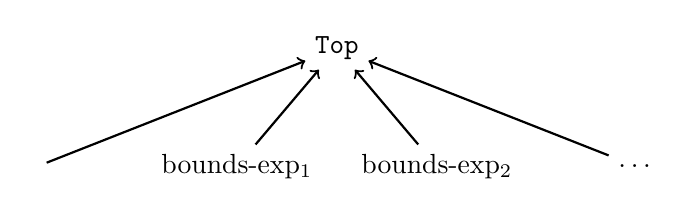
\begin{tikzpicture}[sibling distance=1in]
\node[rectangle, minimum size=8pt]{\texttt{Top}}
  child foreach \name in {\boundsunknown, \var{bounds-exp\textsubscript{1}},
                          \var{bounds-exp\textsubscript{2}}, \ldots}
     {node{\name} edge from parent[<-, thick]};
\end{tikzpicture}
\end{center}
\caption{The lattice of values used in dataflow computation of extent}
\label{fig:extent-dataflow-lattice}
\end{figure}
 
For an assignment to an \arrayptr\ variable, the existing
lattice value for the \arrayptr\ variable is killed, unless
the special conditions described in Section~\ref{section:extent-of-declarations}
are met. 
A new lattice value is generated for the \arrayptr\ variable. If the
assignment declares bounds for the \arrayptr\ variable, the new
lattice value is the bounds expression in the bounds declaration.
Otherwise, it is the value \boundsunknown.

A declaration of a variable is handled similarly to an assignment,
except that there will not be any lattice value to kill. Lexical hiding
of variables involved in bounds declarations is not permitted. If the
declaration declares bounds for the \arrayptr\ variable, the
new lattice value is the bounds expression in the bounds declaration.
Otherwise, it is the value \boundsunknown.

A variable going out of scope kills any existing lattice values in which
that variable occurs.

At control-flow split points, the lattice values for the
\arrayptr\ variables flow to all branches of the split. The
propagation is dataflow-sensitive but not control-flow sensitive. At
control-flow join points, the lattice values are unioned (moving upward
in the lattice). If the lattice values for an \arrayptr\
variable are not the same, the resulting value is \texttt{Top}.

\section{Bounds declarations and loops}

Loops often operate on variables declared outside of loops. They may
read the variables and then update the variables. When these variables
are \arrayptr\ variables they must have bounds and the bound
must be loop invariants.

The common case is that the bounds expression is invariant across all
iterations of the loop. The earlier \code{sum} example illustrates
this. The variable \code{current} is declared with bounds before a
loop. The loop modifies \code{current}, but the bounds for
\code{current} do not change:

\begin{lstlisting}
/* sum integers stored between start and end, where end is not included */
int sum(array_ptr<int> start where start : bounds(start, end), array_ptr<int> end)
{ 
    int sum = 0;
    array_ptr<int> current : (start, end) = start;

    while (current < end) {
       sum = *current;
       current += 1; // bounds do not need to be redeclared here.
    }
}
\end{lstlisting}

A programmer can declare bounds expressions that change on each
iteration of the loop. This may be necessary if an \arrayptr\
variable is modified to point to different memory during a loop
iteration. It also may be desirable for performance reasons. In either
case, there needs to be a loop-invariant bounds declaration.

The following example illustrates this. It is an implementation of
lexicographic comparisons of two arrays, using one pointer to scan each
array. The bounds at the variable declarations serve as loop invariant
bounds. The lower bounds for a variable are declared using the variable
itself, to reduce register pressure in the loop. This can enable
compilers to generate better code. Note that an optimizing compiler will
eliminate the runtime bounds checks easily.

\begin{lstlisting}
/* lexicographic comparison of two arrays of integers */
int compare(array_ptr<int> x : bounds(x, x_end), 
            array_ptr<int> y : bounds(y, y_end)
            array_ptr<int> x_end, array_ptr<int> y_end)
{ 
  while (x < x_end && y < y_end) {
    if (*x == *y) { // bounds check: x >= x && x < x_end; easily
                    // optimizable.
                    // bounds check: y >= y && y < y_end; easily
                    // optimizable.
      x++;
      y++;
    }
    else if (*x < *y) { // bounds checks here are easily optimizable too.
      return -1;
    }
    else {
      return 1;
    }
  }
  if (x == x_end && y == y_end) {
    return 0;
  }
  else if (x != x_end) {
    return 1;
  }
  else {
    return -1; 
  }
}
\end{lstlisting}

